\chapter{Drawings of the prototypes and test bench}
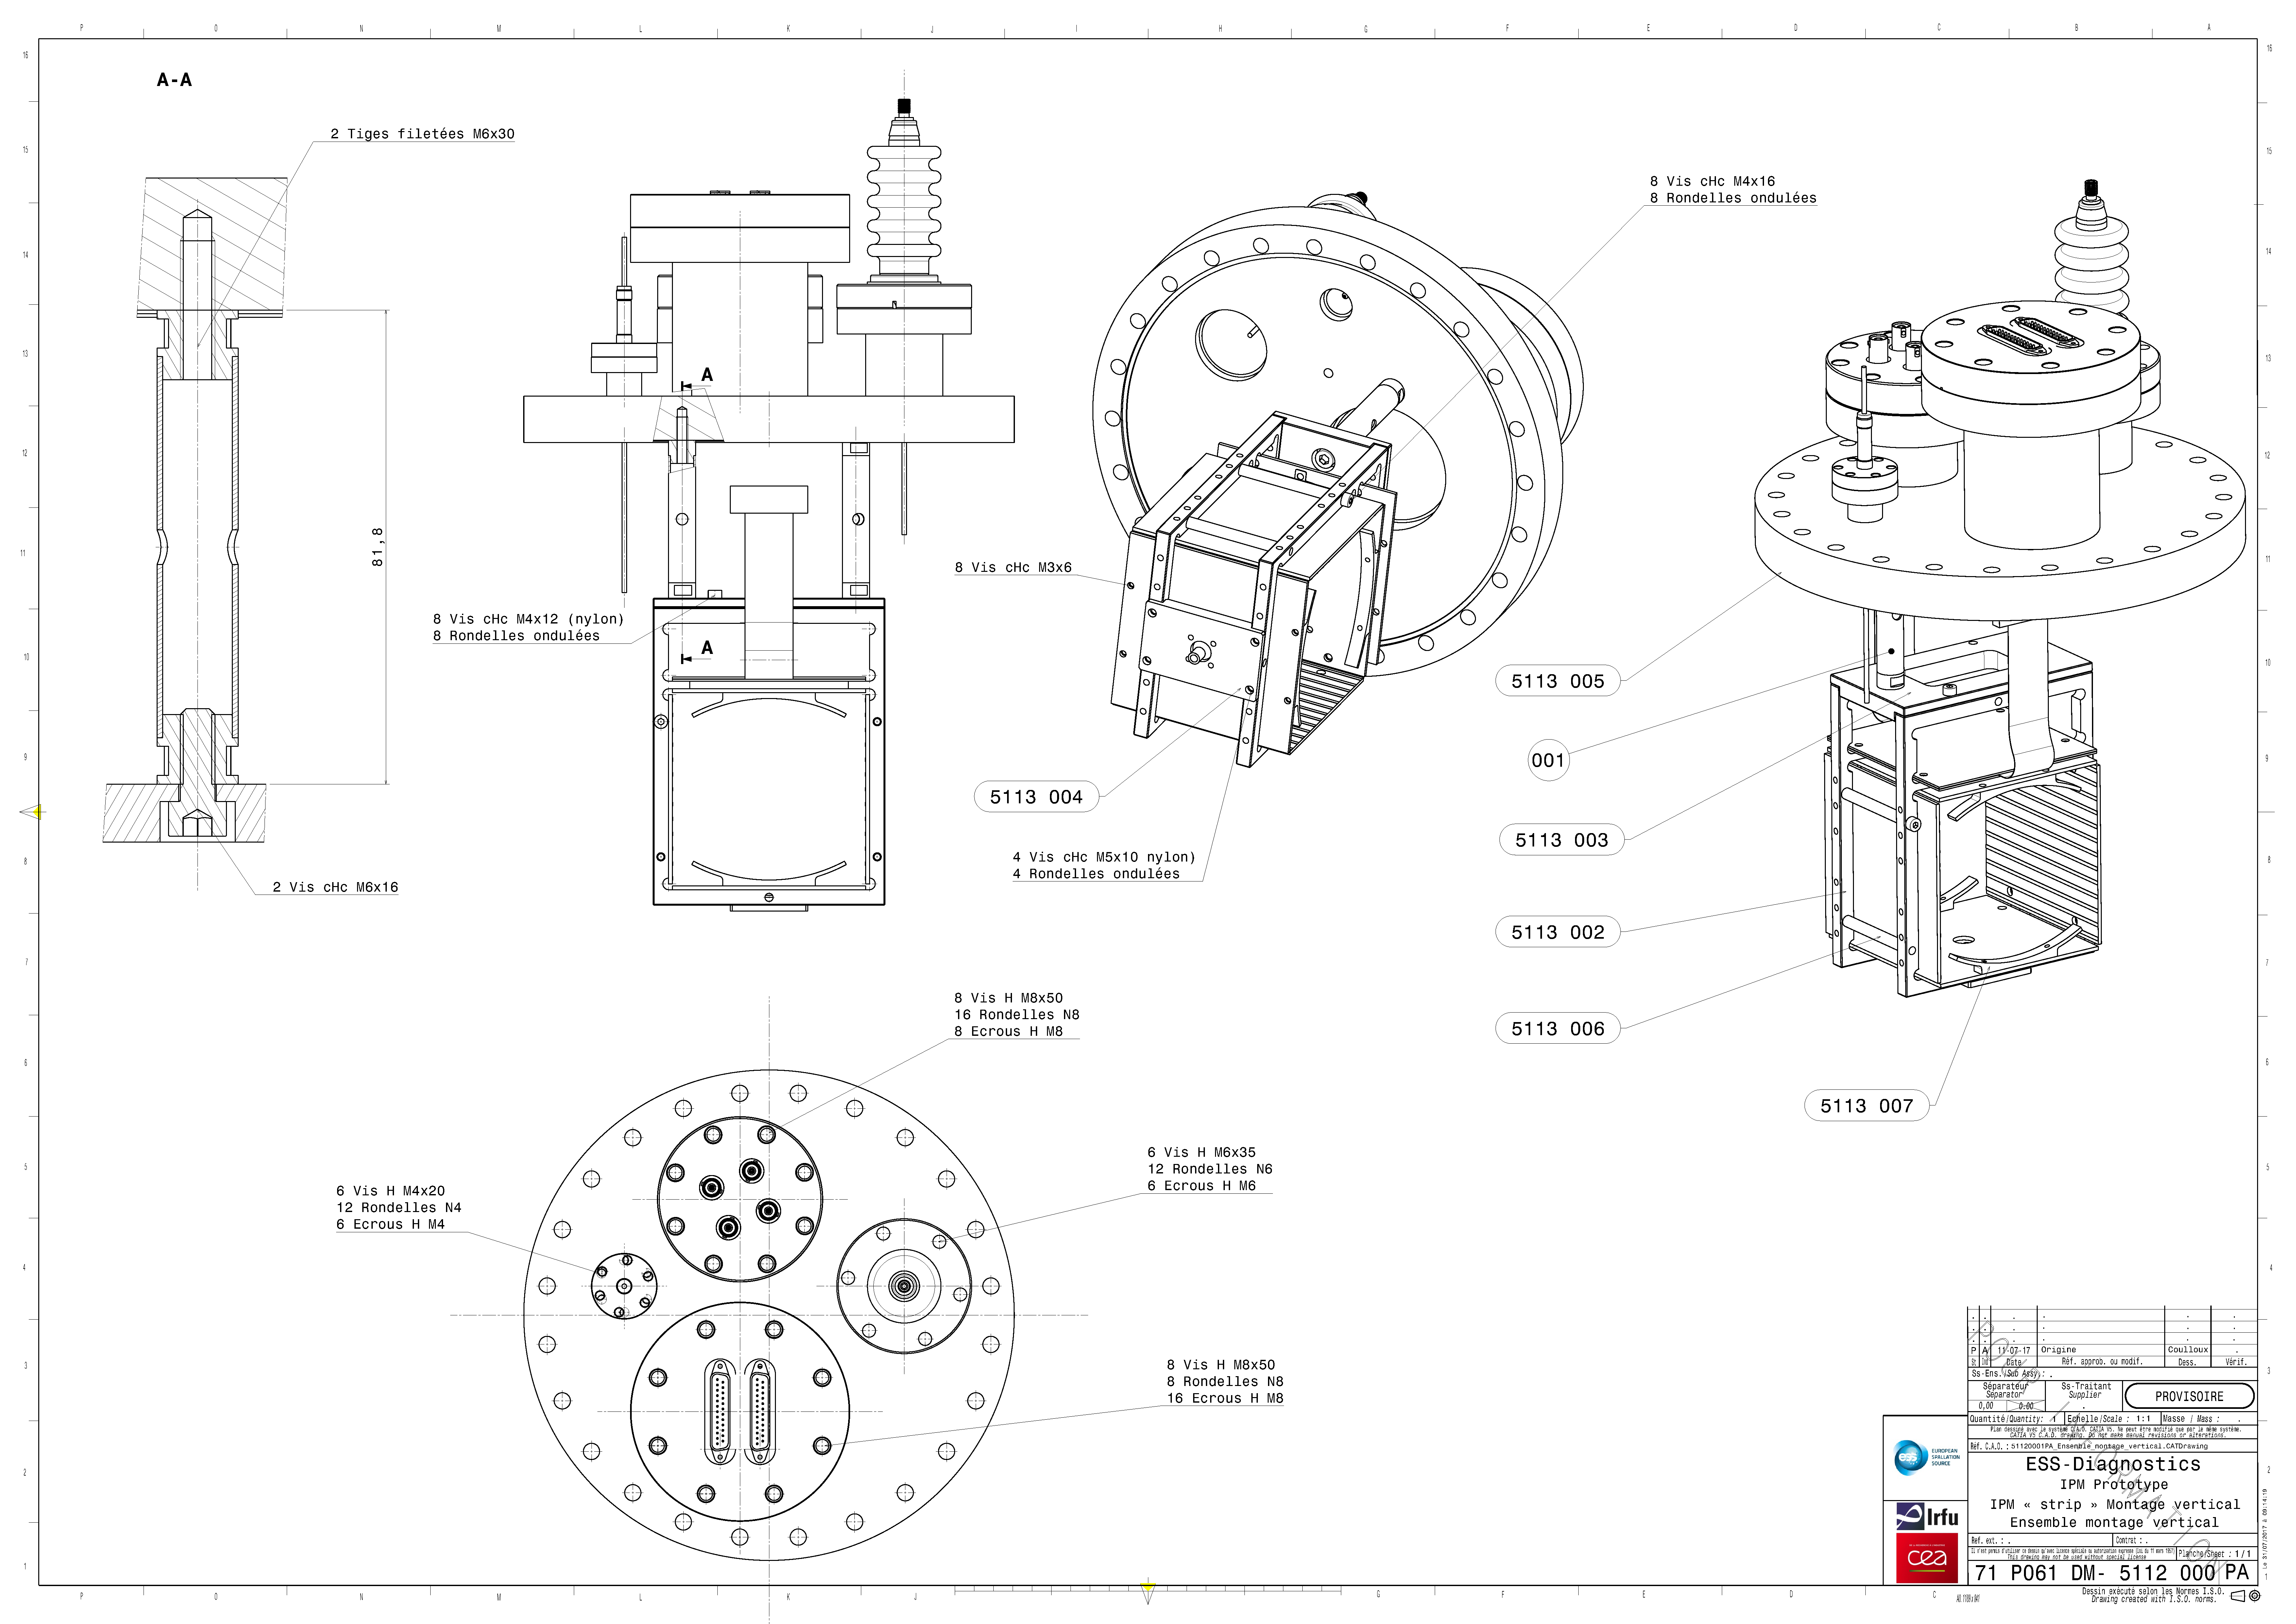
\includepdf[angle=90]{00_Appendix/anx000_IPMstrip1}
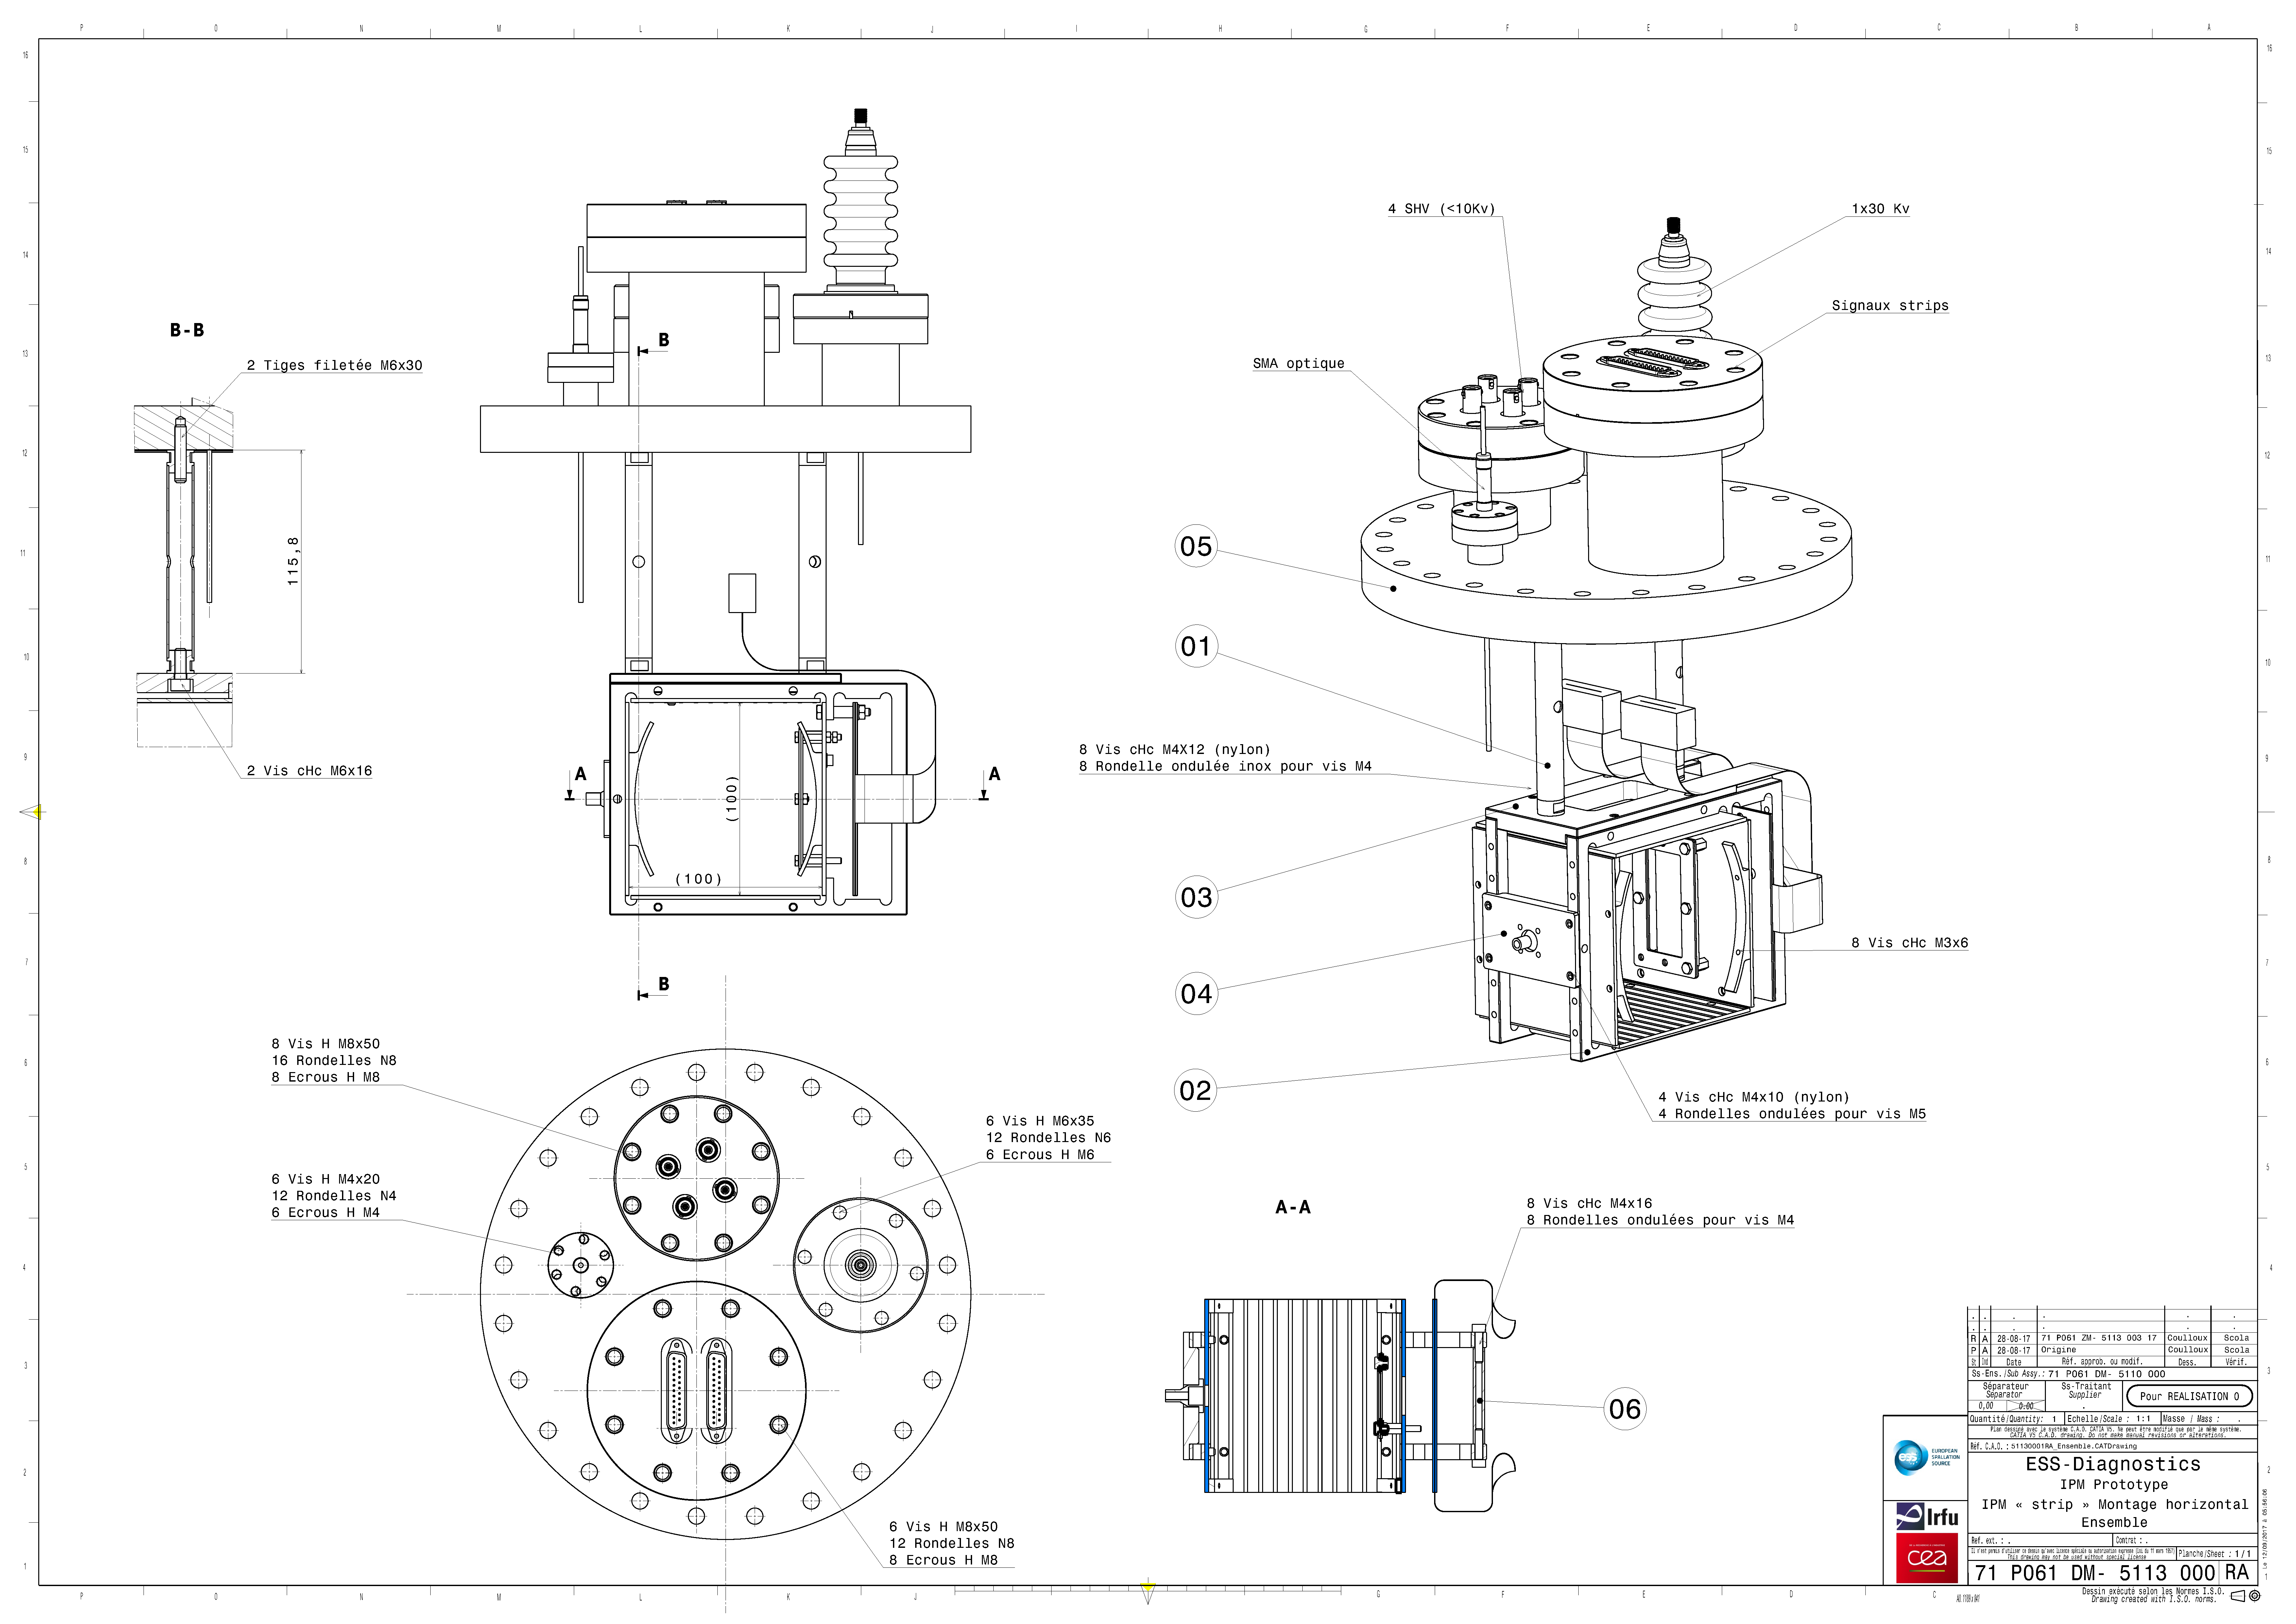
\includepdf[angle=90]{00_Appendix/anx000_IPMstrip2}
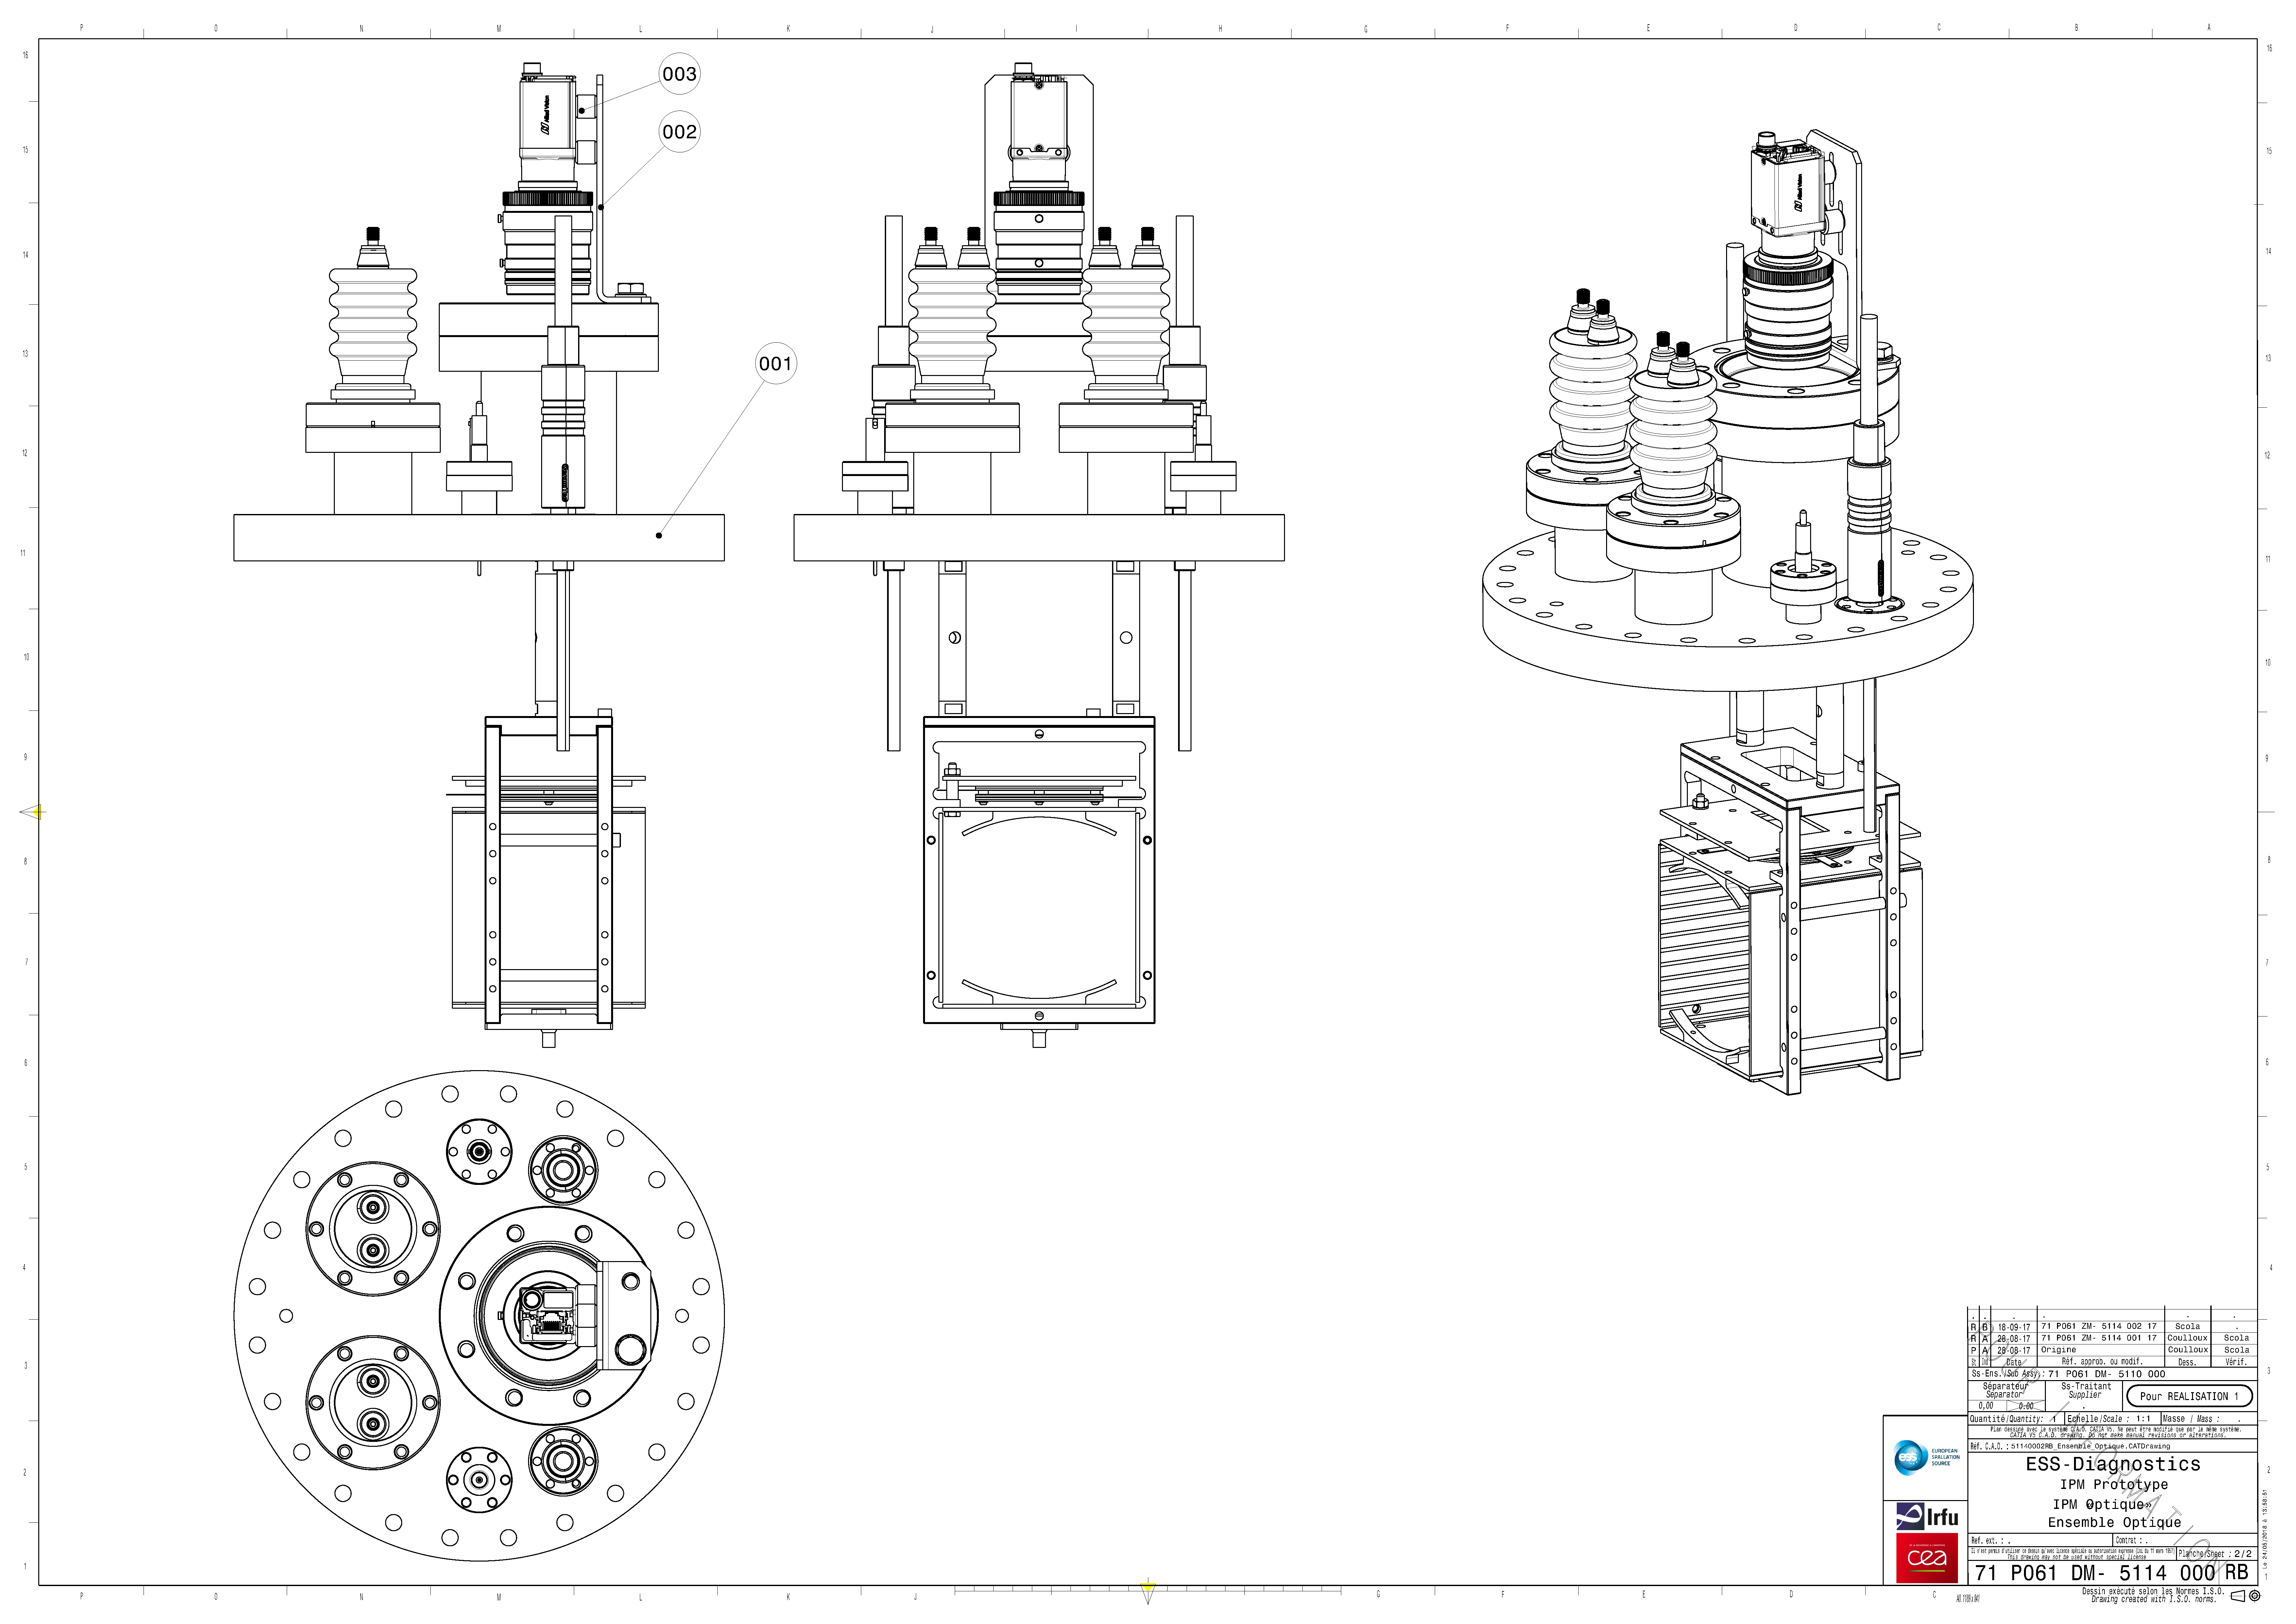
\includepdf[angle=90]{00_Appendix/anx000_IPMoptic1}
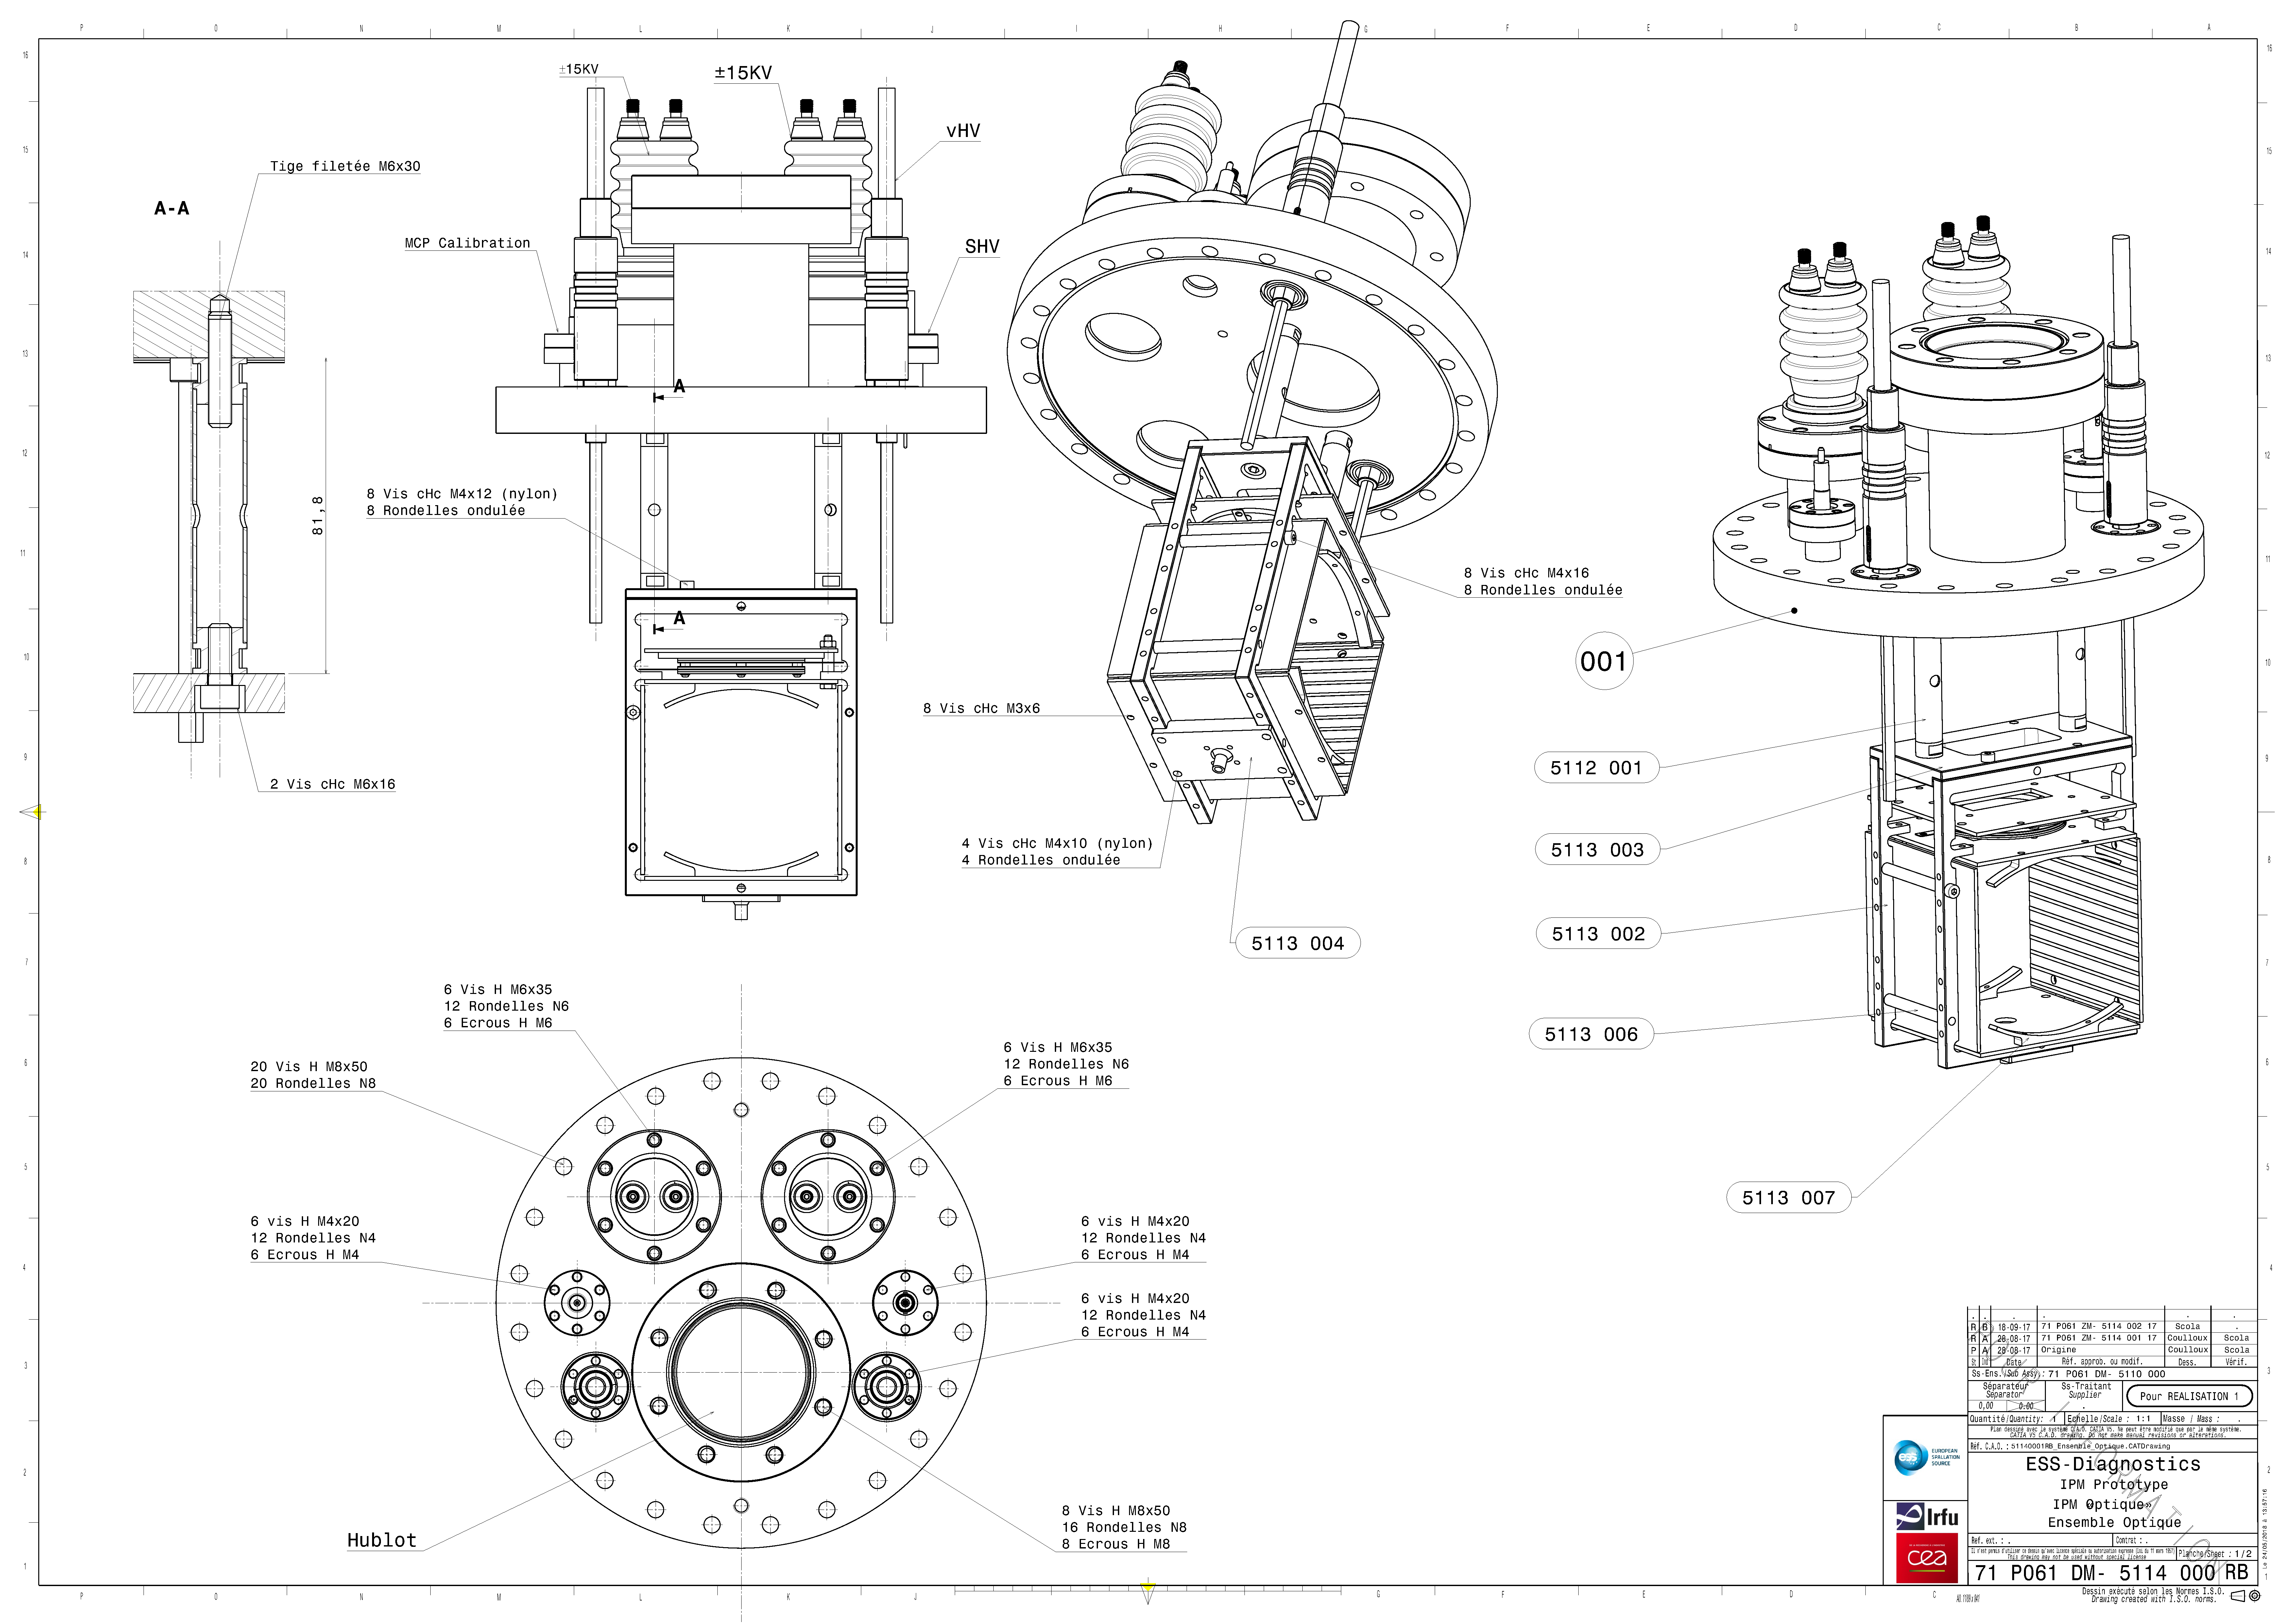
\includepdf[angle=90]{00_Appendix/anx000_IPMoptic2}
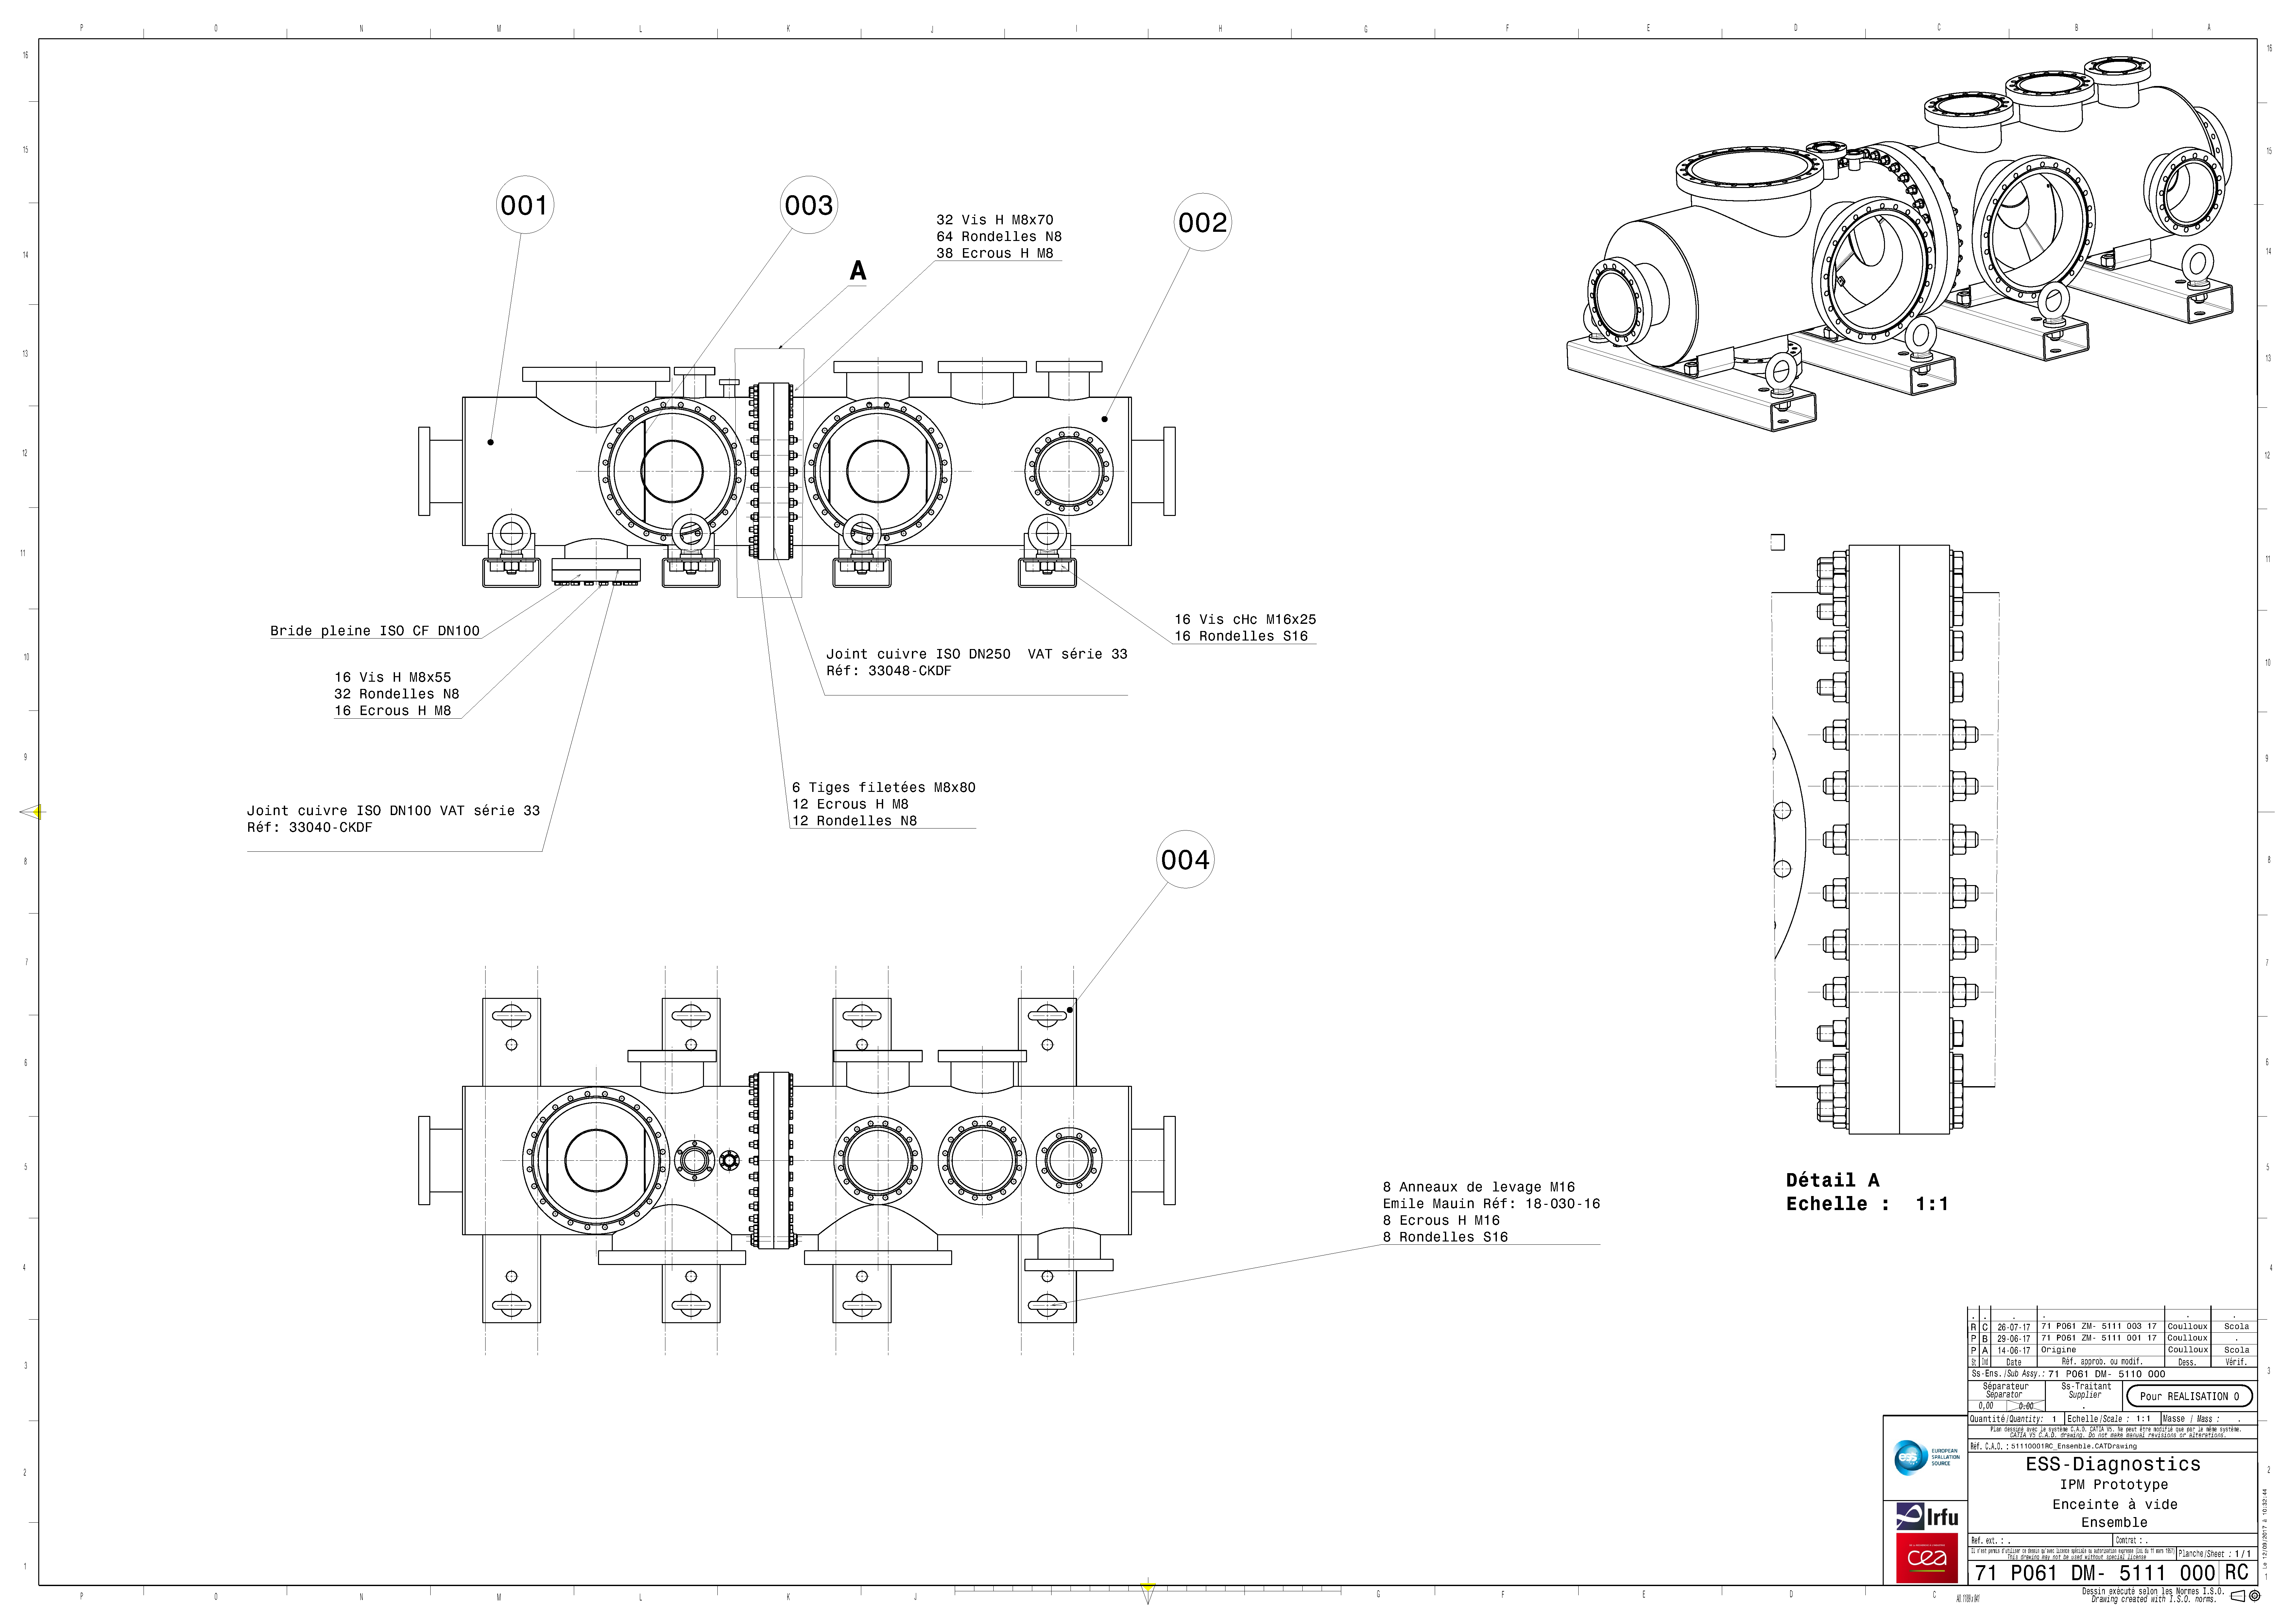
\includepdf[angle=90]{00_Appendix/anx000_tb1}
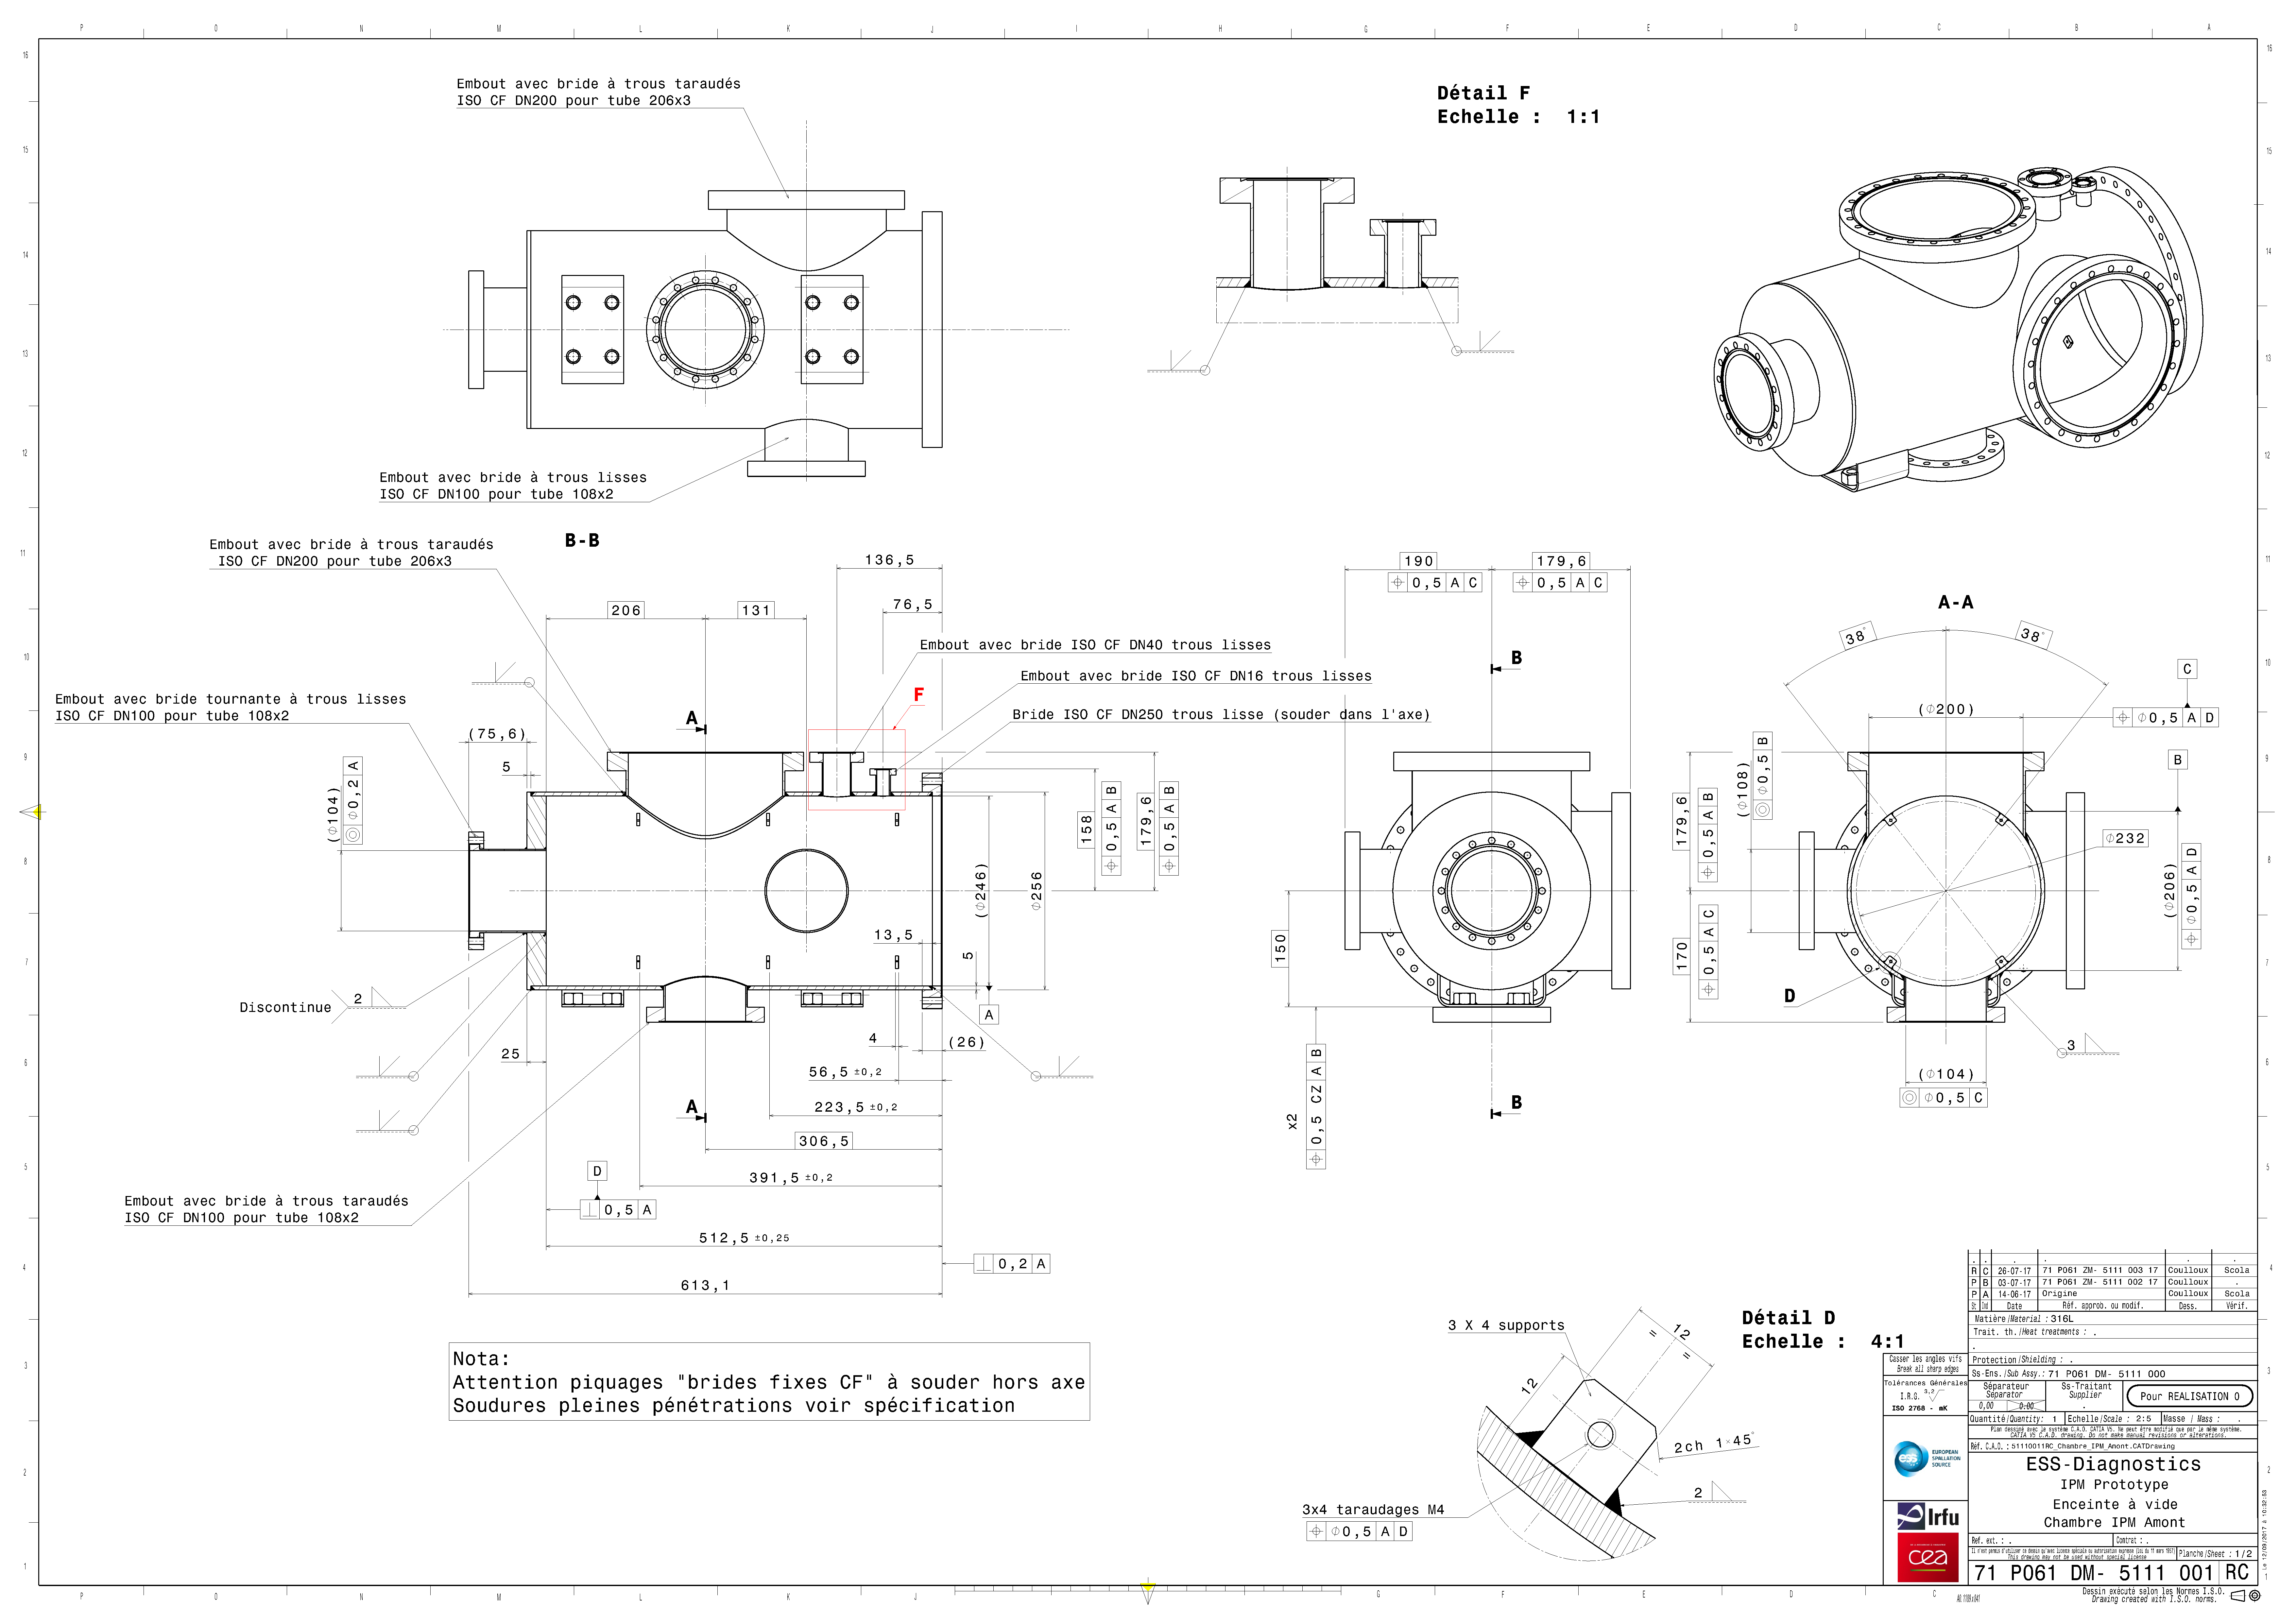
\includepdf[angle=90]{00_Appendix/anx000_tb2}
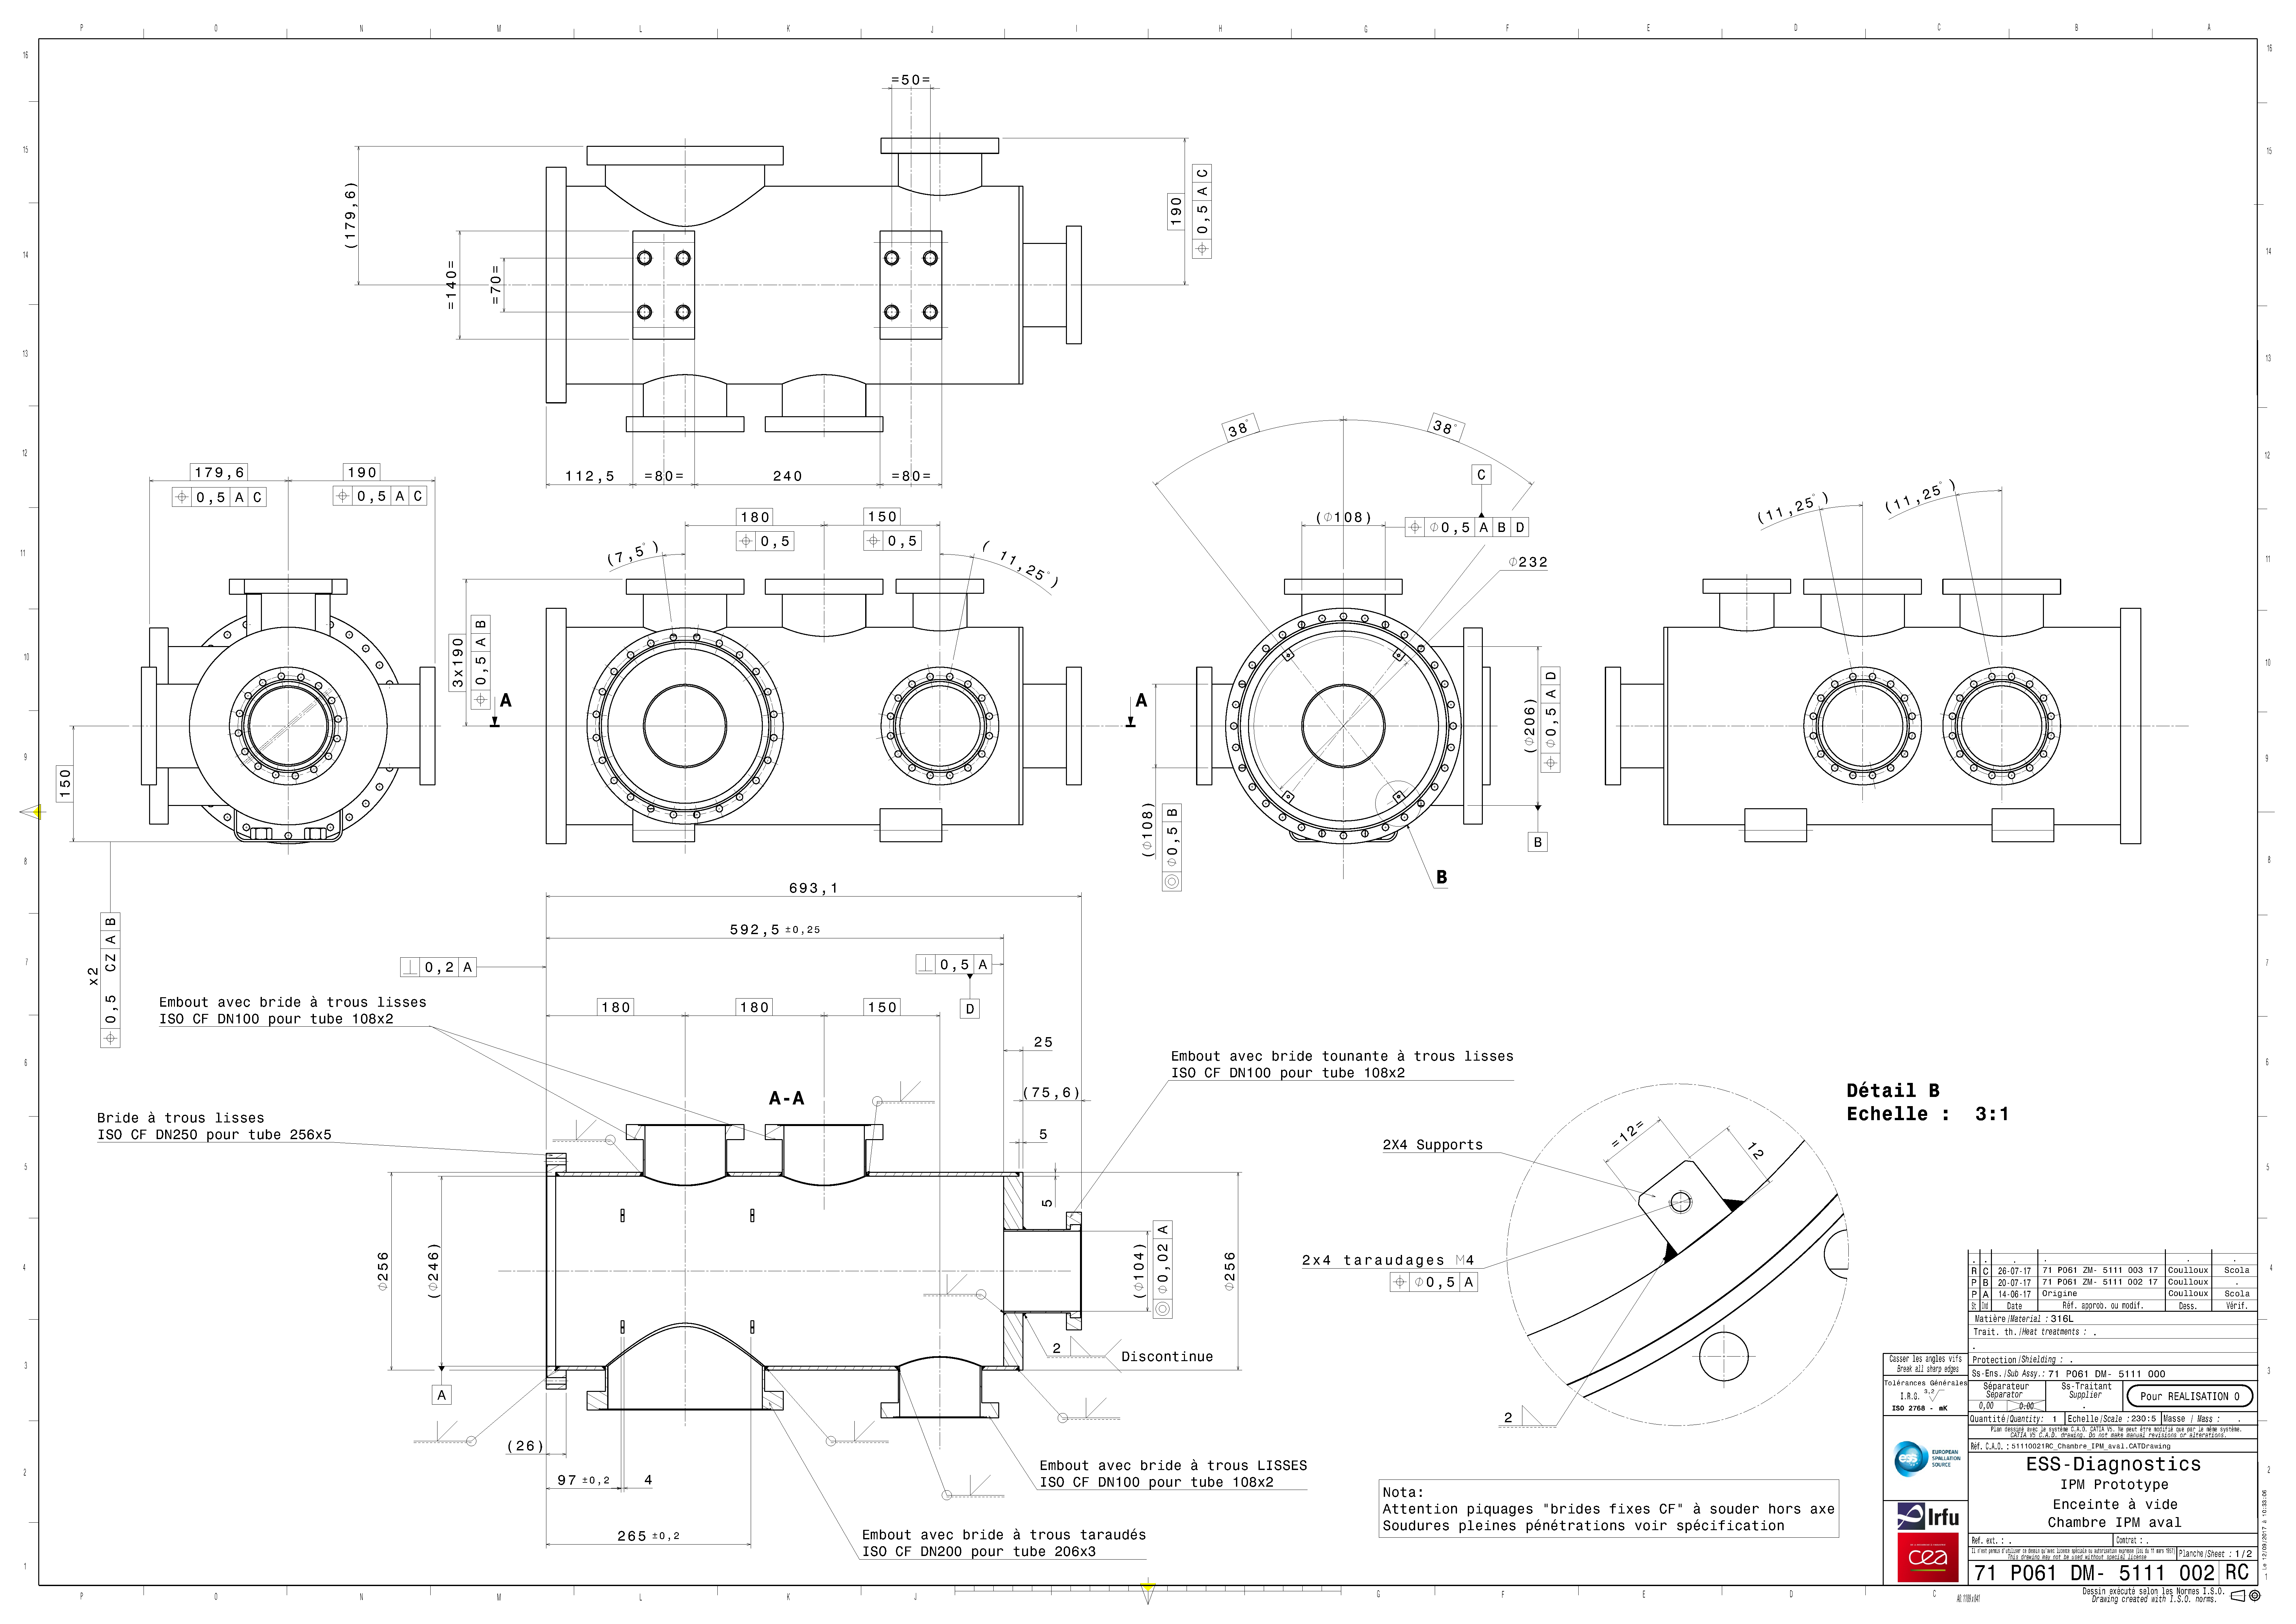
\includepdf[angle=90]{00_Appendix/anx000_tb3}

\chapter{Summary of COMSOL results}
\label{anx:COMSOL}
This appendix presents the most important results of the COMSOL simulations, especially the effects of the different elements (power supply configurations, shielding disks, field correctors and curved electrodes) on the extraction field uniformity.
For each case the following graphs are plotted:
\begin{enumerate}
  \item Longitudinal field plot. The COMSOL model is sliced in the longitudinal direction. For each slice and for each field components, the quadratic mean is computed in the middle of the IPMs. The means are normalized by the expected field in case of the IPM is perfect ($\frac{\Delta V}{d_{IPM}}$).
  \item Results of a particle tracking. The particles are drawn in the middle of the IPM and their final positions are recorded on the readout plane.
  \item Results of particle tracking simulations for several locations in the IPM. The absolute error on the beam position and the relative error on the beam size is then computed for several transversal locations.
\end{enumerate}

Brief descriptions of the different setups used in the simulations are reported in Table \ref{anx:tab:recap_simu}.
\begin{table}[!h]
  \centering
  \caption[Summary of the different cases simulated with COMSOL]{Summary of the different cases simulated with COMSOL.}
  \label{anx:tab:recap_simu}
  \begin{tabularx}{\linewidth}{lXXXX}
    \toprule
    Simulation & Field      & Disks & Correctors & Curved \\
    \midrule
    1          & Asymmetric & No    & No         & No     \\
    2          & Asymmetric & No    & Yes        & No     \\
    3          & Asymmetric & No    & Yes        & Yes    \\
    4          & Asymmetric & Yes   & No         & No     \\
    5          & Asymmetric & Yes   & Yes        & No     \\
    6          & Asymmetric & Yes   & Yes         & Yes    \\
    7          & Symmetric  & No    & No         & -      \\
    8          & Symmetric  & No    & Yes        & -      \\
    9          & Symmetric  & Yes   & No         & -      \\
    10         & Symmetric  & Yes   & Yes        & -      \\
    \bottomrule
  \end{tabularx}
\end{table}
% \section{IPM in asymmetric mode without correction}
% This is most basic setup, in this case the IPMs are

% The profile is

% \section{IPM in asymmetric mode with field correctors only}

% \section{IPM in asymmetric mode with field correctors and curved electrodes}

% \section{IPM in asymmetric mode with disks only}

% \section{IPM in asymmetric mode with disks and field correctors}

% \section{IPM in asymmetric mode with disks and curved electrodes}

% \section{IPM in symmetric mode without correction}
% \section{IPM in symmetric mode with field correctors only}
% \section{IPM in symmetric mode with disks only}
% \section{IPM in symmetric mode with disks and field correctors}


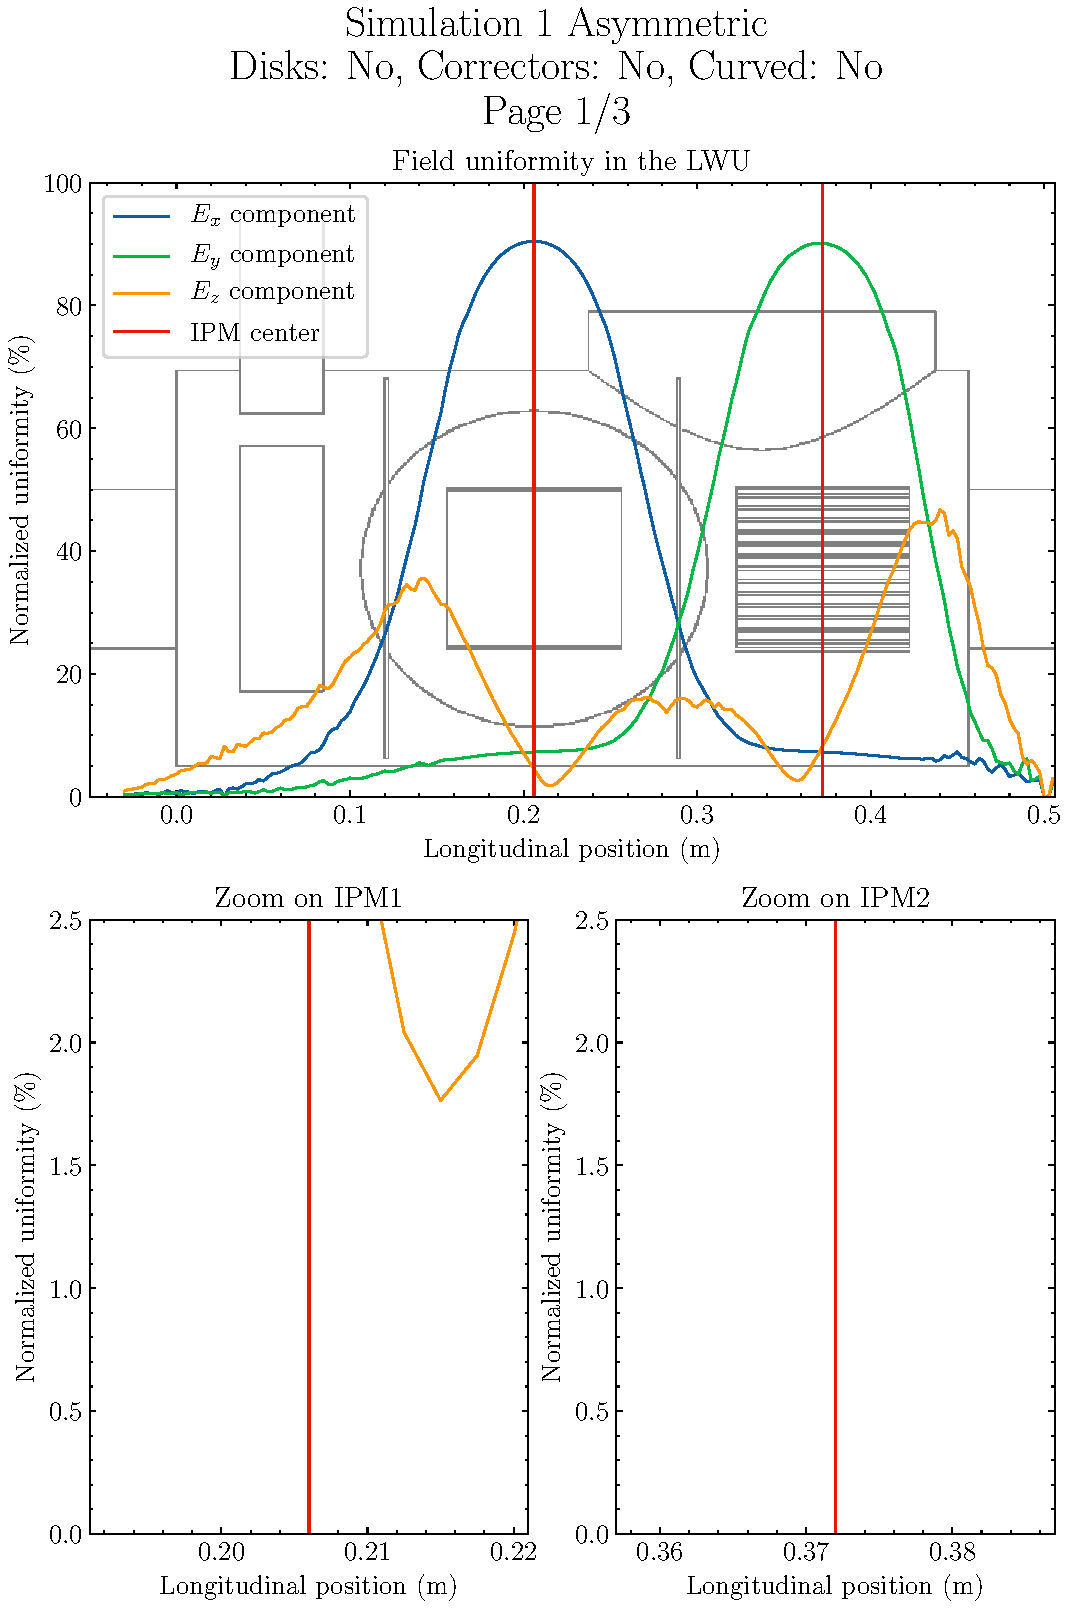
\includepdf[pages=1-]{00_Appendix/anx000_COMSOL_sum_v3.pdf}

%\chapter{Drawings of the final design}

\chapter{Conference proceeding and scientific documents}
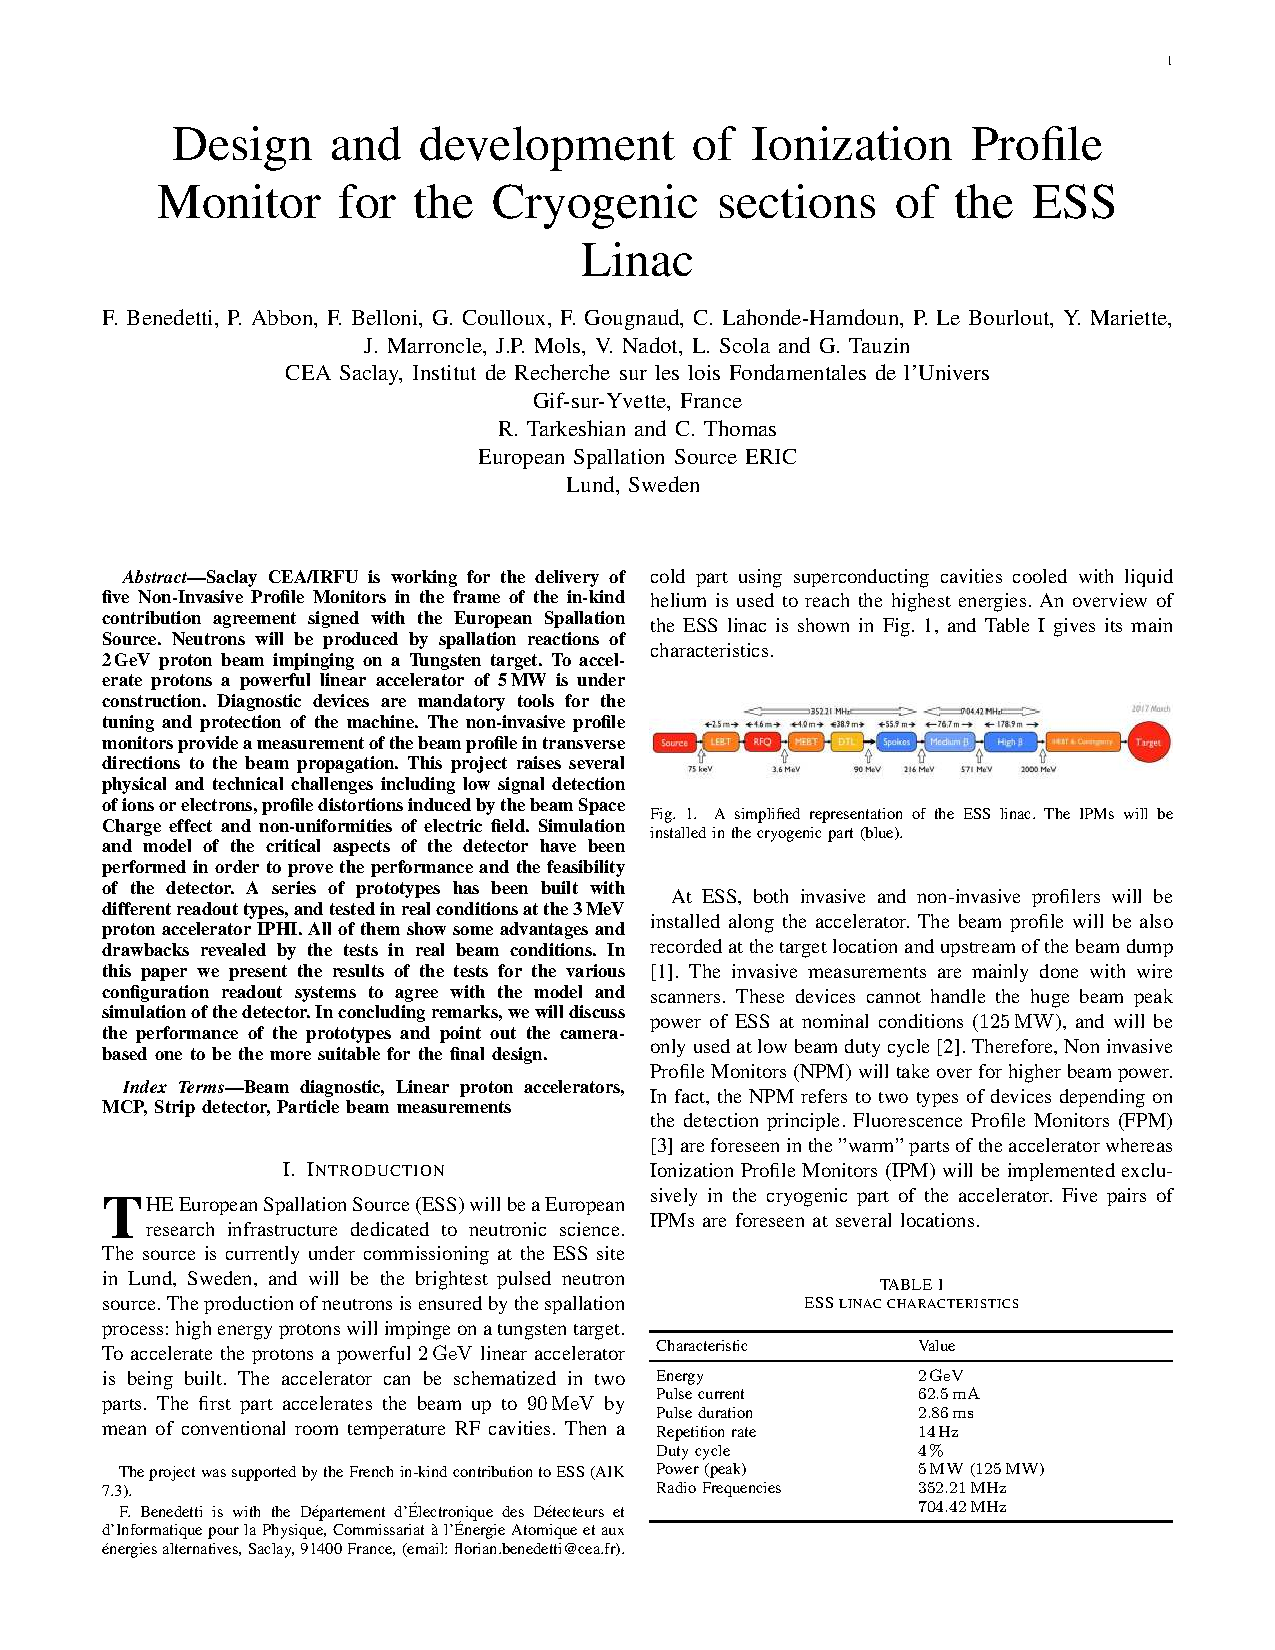
\includepdf[pages=1-]{00_Appendix/ANIMMA_2019_2}

%\chapter{More on ESS conditions}

%\chapter{TraceWin IPHI}